%%%%%%%%%%%%%%%%%%%%%%%%%%%%%%%%%%%%%%%%%%%%%%%%%%%%%%%%%%%%%%%%%%%%%%%%%%%%%%
%                       NmapSI4 Latex Documentation                          %
%              copyright: Antonio Salvucci <s4lb04@gmail.com>                %
%%%%%%%%%%%%%%%%%%%%%%%%%%%%%%%%%%%%%%%%%%%%%%%%%%%%%%%%%%%%%%%%%%%%%%%%%%%%%%

%%%%%%%%%%%%%%%%%%%%%%%%%%%%%%%
%%%%%%%%%%%%%%%%%%%%%%%%%%%%%%%
\chapter{Indice dei contenuti}
\label{ch:Contents}
%%%%%%%%%%%%%%%%%%%%%%%%%%%%%%%
%%%%%%%%%%%%%%%%%%%%%%%%%%%%%%%

%%%%%%%%%%%%%%%%%%%%%%%%%%%
\section{Introduzione}
\label{sec:ContentsIntro}
%%%%%%%%%%%%%%%%%%%%%%%%%%%

%NmapSI4 \`e una GUI completa, realizzata in Qt, per Nmap, con l'obiettivo di 
%dare maggiore padronanza agli utenti di questo potente strumento di analisi.

%%%%%%%%%%%%%%%%%%%%%%%%%%%%%%%
\section{Schermata Principale}
\label{sec:ContentsMain}
%%%%%%%%%%%%%%%%%%%%%%%%%%%%%%%

\begin{figure}[h]
  \centering
  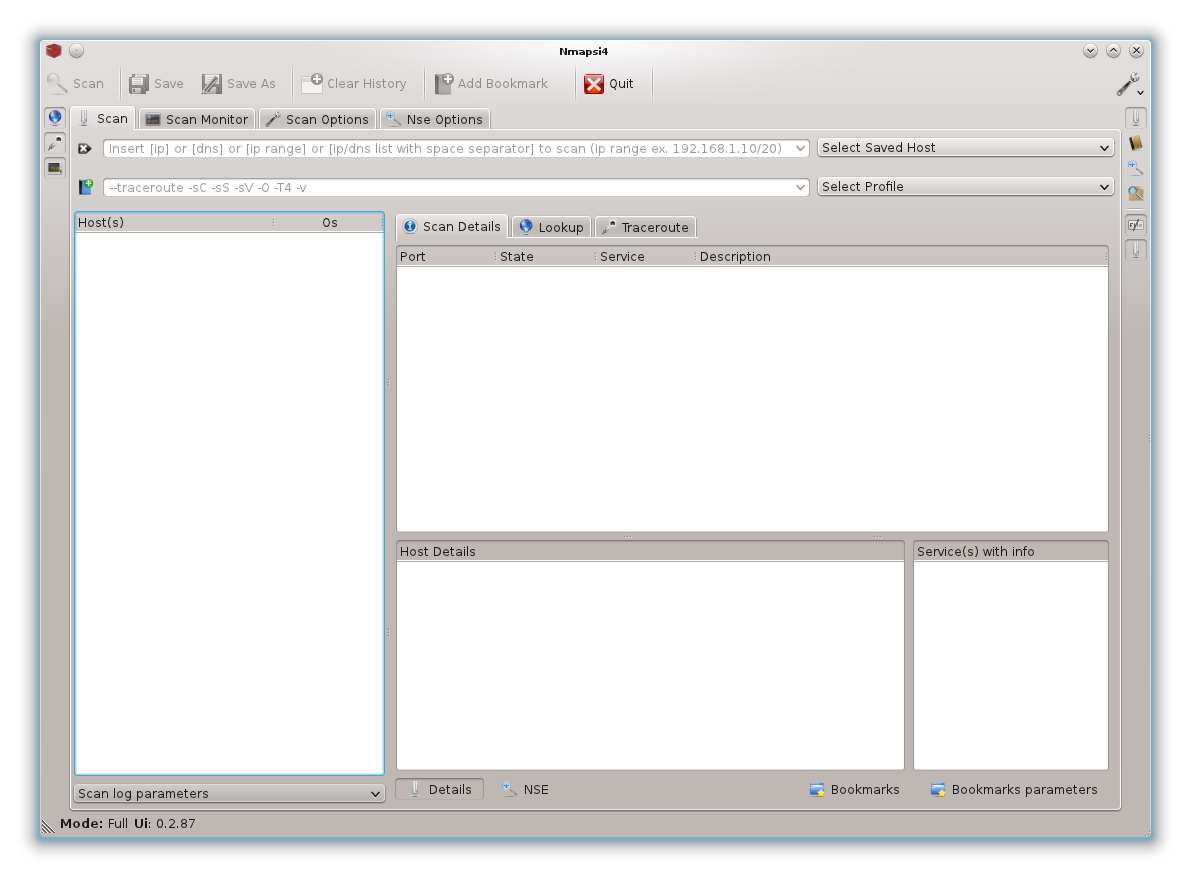
\includegraphics[width=0.65\textwidth]{main}
  \caption{Dettagli di scansione}
  \label{fig:ContentsMainScanDetails}
\end{figure}
Questa \`e la schermata principale di NmapSI4, possiamo notare alcuni elementi:
\begin{itemize}
\item Barra dei menu
\item Barra di strumenti
\item Form di inserimento host, ip o dns per la scansione
\item Form di inserimento per i parametri di scansione
\item Schermata dei risultati
\item Barra di stato
\end{itemize}
Per iniziare una scansione inserire un host, ip o dns e cliccare sul pulsante 
``Scan''. Al termine della scansione, vengono visualizzati i risultati nella 
schermata dei risultati. Sulla barra di stato \`e possibile vedere con quali 
diritti \`e in esecuzione NmapSI4 insieme alla sua versione software ed 
insieme alla versione software per Nmap.

%%%%%%%%%%%%%%%%%%%%%%%%%%
\section{Scansione}
\label{sec:ContentsScan}
%%%%%%%%%%%%%%%%%%%%%%%%%%

Questa sezione riguarda i pulsanti presenti sotto la schermata dei risultati.

\subsection{Dettagli di scansione}
\label{sec:ContentsScanDetails}

\begin{figure}[h]
  \centering
  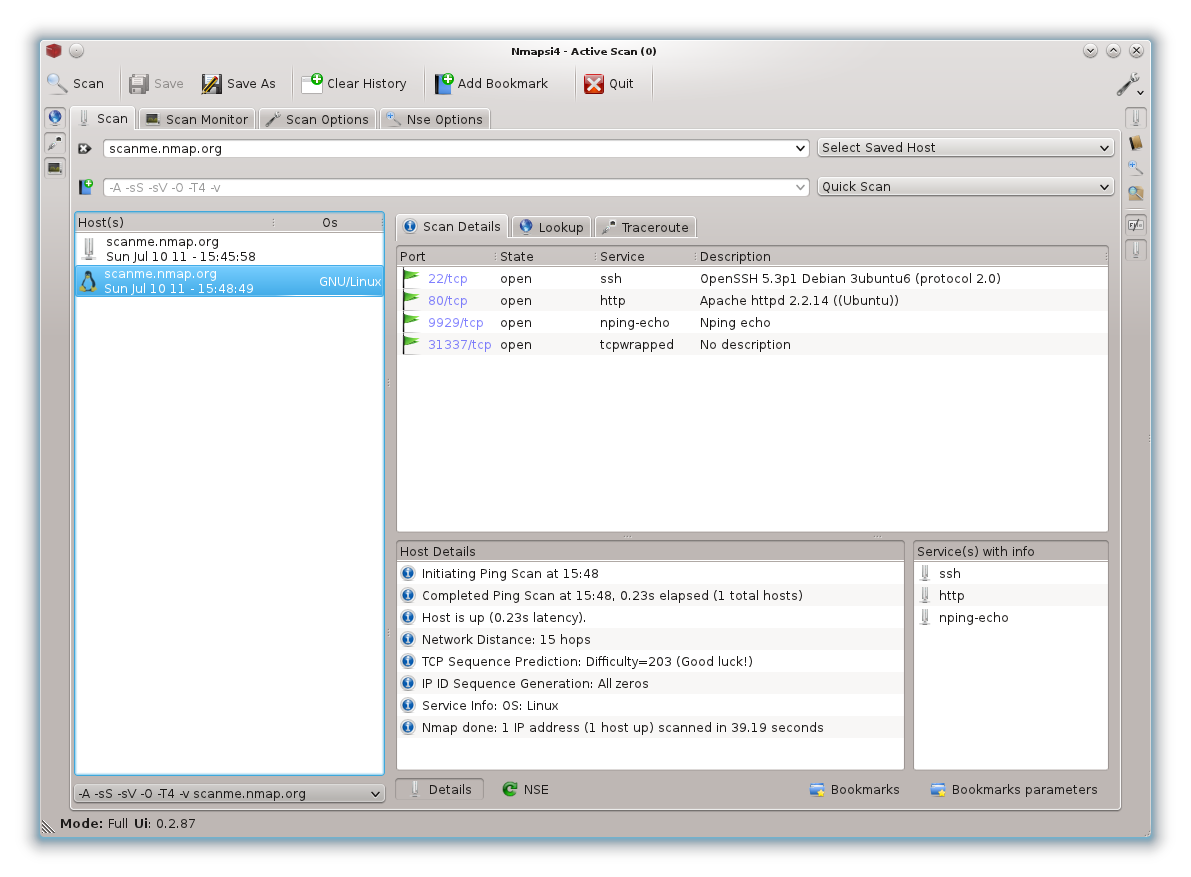
\includegraphics[width=0.65\textwidth]{11scan_details}
  \caption{Dettagli di scansione}
  \label{fig:ScanDetails}
\end{figure}
Qui vengono elencati i risultati della scansione, e nello specifico: la porta 
del servizio, lo stato della porta, il tipo di servizio ed una breve descrizione.

\subsection{Nmap script}
\label{sec:NmapScript}

\begin{figure}[h]
  \centering
  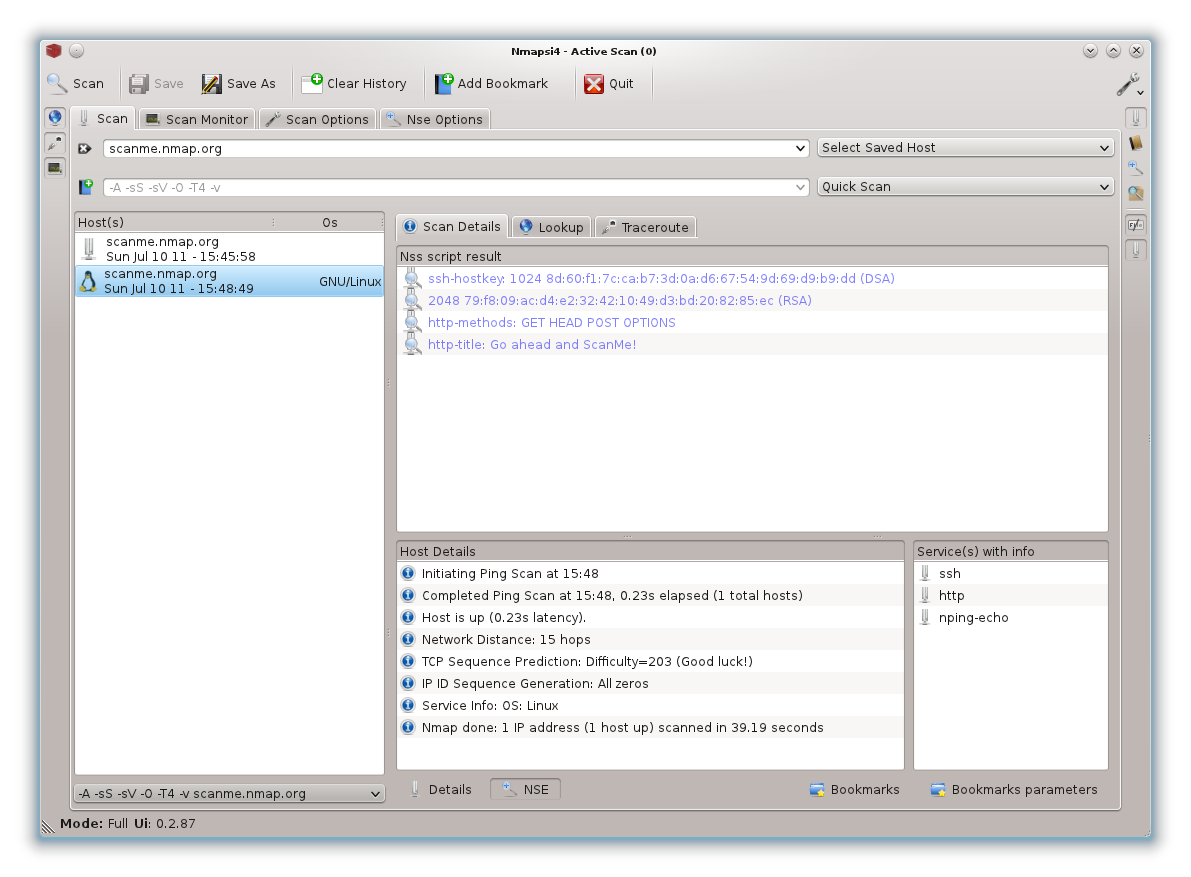
\includegraphics[width=0.65\textwidth]{12nss_result}
  \caption{Nmap script}
  \label{fig:NmapScript}
\end{figure}
Qui vengono mostrati dei risultati in base a degli script presenti nella suite 
Nmap. Per ulteriori informazioni rimandiamo al capitolo specifico della 
\href{http://nmap.org/book/nse.html}{guida Nmap}.

\subsection{Host info}
\label{sec:HostInfo}

\begin{figure}[h]
  \centering
  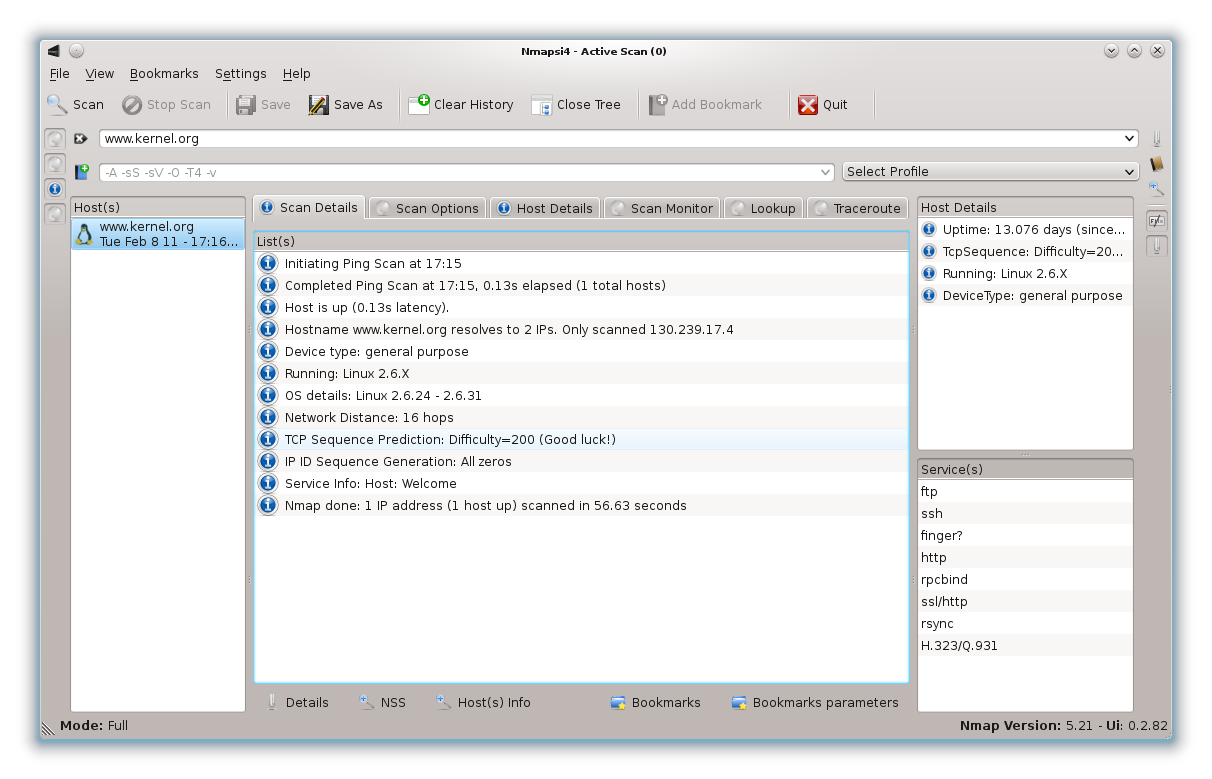
\includegraphics[width=0.7\textwidth]{13host_info}
  \caption{Host info}
  \label{fig:HostInfo}
\end{figure}
Qui sono presenti dettagli relativi alla scansione, come l'ora di inizio, la 
durata della scansione ed altre informazioni utili.

\subsection{Preferiti}
\label{sec:Bookmarks}

\begin{figure}[h]
  \centering
  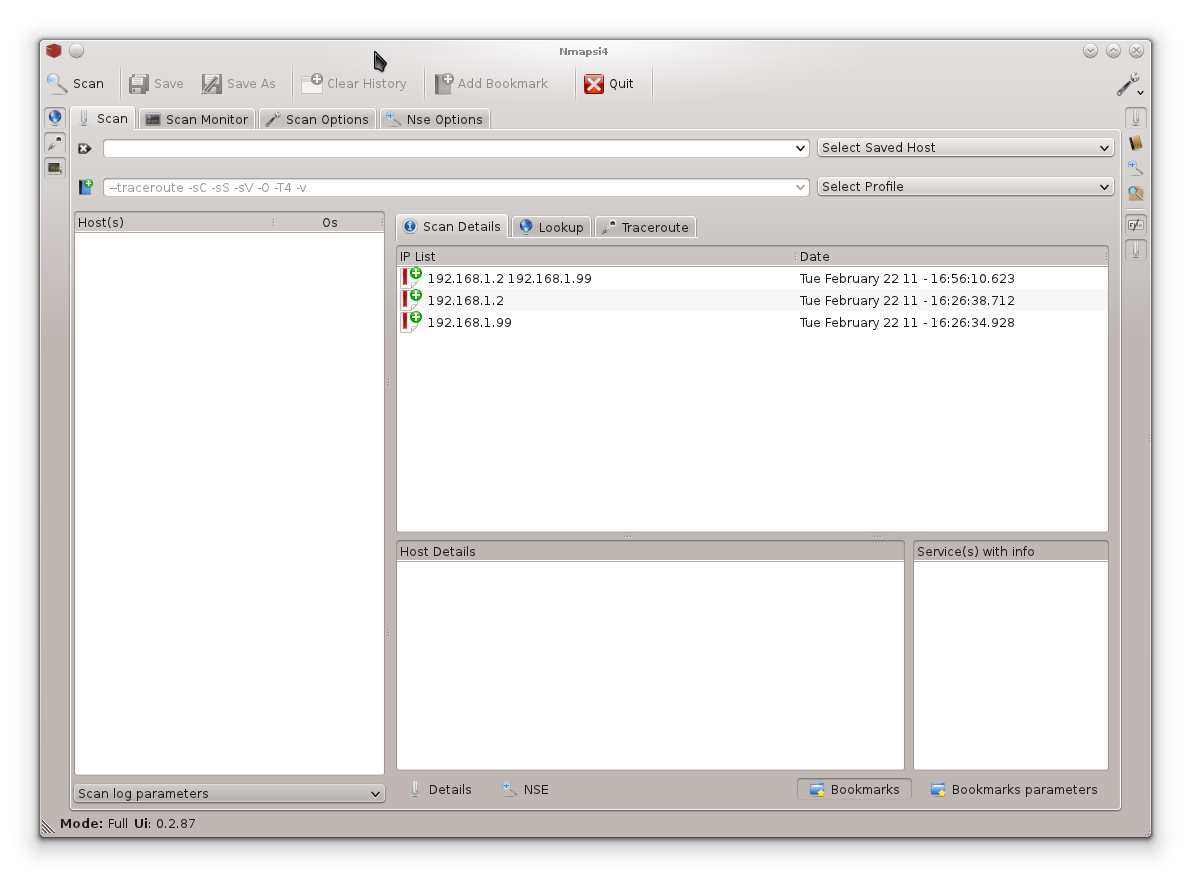
\includegraphics[width=0.7\textwidth]{14bookmarks}
  \caption{Preferiti}
  \label{fig:Bookmarks}
\end{figure}
Qui possiamo mantenere i nostri bersagli preferiti. La schermata ci mostra l'ip 
o il nome host e la data di memorizzazione.

\subsection{Parametri dei preferiti}
\label{sec:BookmarksParameters}

Qui possiamo visualizzare i parametri di scansione dei preferiti memorizzati.
\begin{figure}[h]
  \centering
  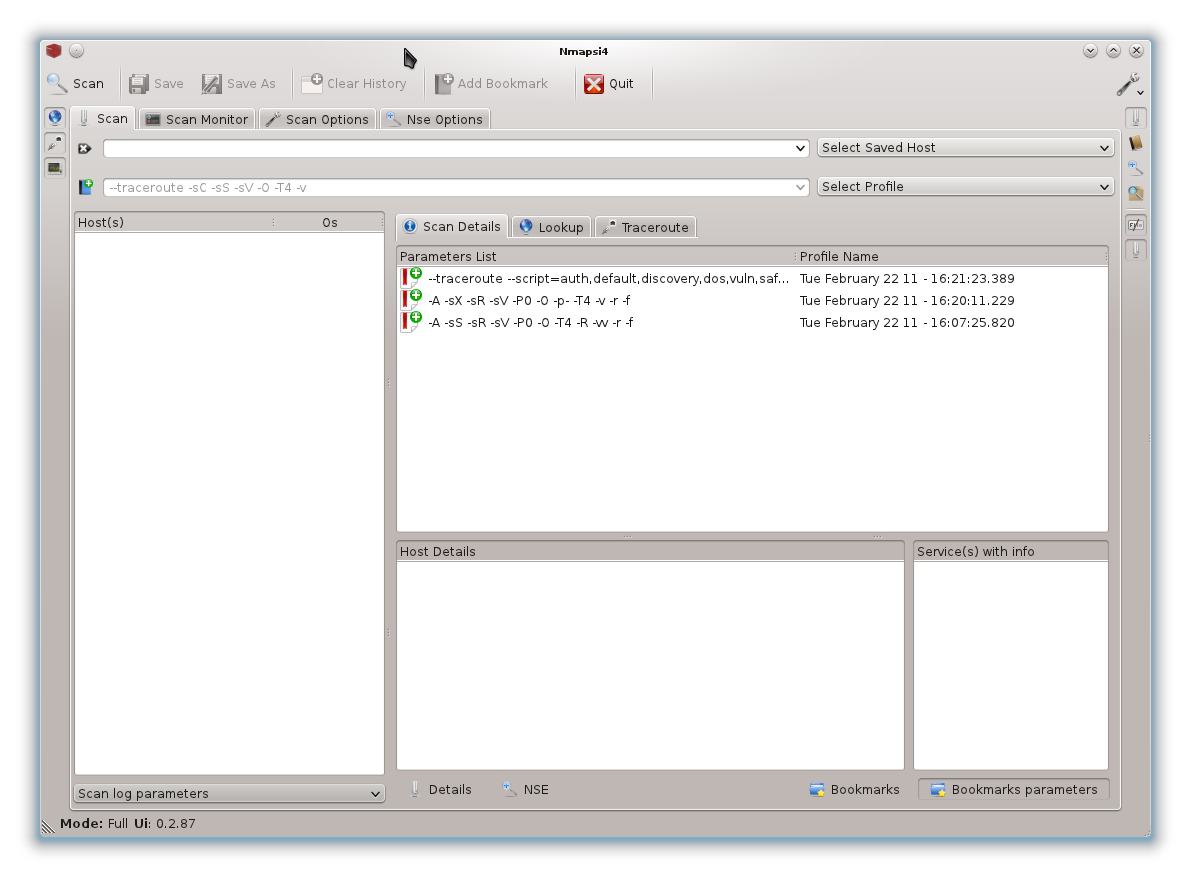
\includegraphics[width=0.7\textwidth]{15bookmarks_parameters}
  \caption{Parametri dei preferiti}
  \label{fig:BookmarksParameters}
\end{figure}


%%%%%%%%%%%%%%%%%%%%%%%%%%%%%%%%%
\section{Opzioni di scansione}
\label{sec:ScanOptions}
%%%%%%%%%%%%%%%%%%%%%%%%%%%%%%%%%

In questa sezione \`e possibile cambiare i parametri di scansione. Per applicare 
i cambiamenti \`e necessario usare il pulsante in basso ``Applica''.

\subsection{Scansione}
\label{sec:ScanParameters}

\begin{figure}[h]
  \centering
  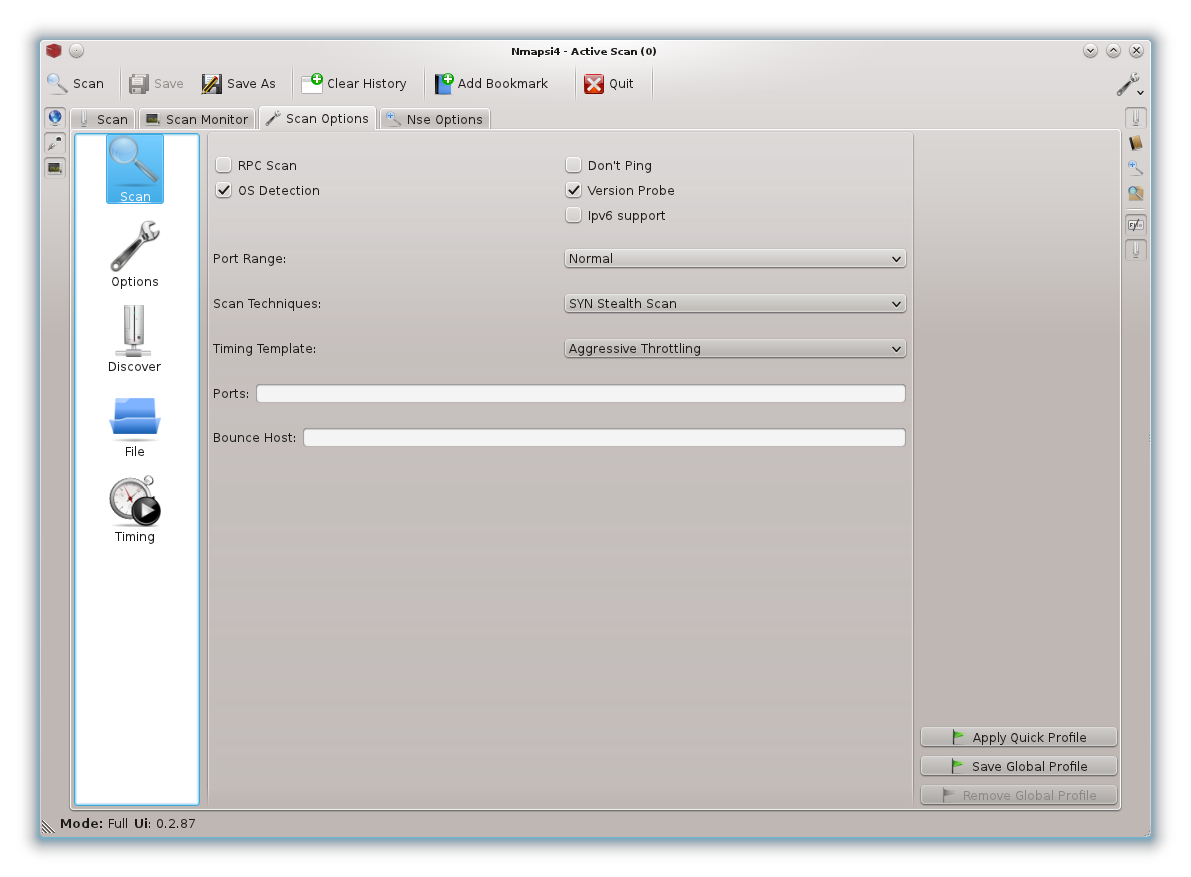
\includegraphics[width=0.7\textwidth]{21scan_options}
  \caption{Scansione}
  \label{fig:ScanParameters}
\end{figure}
Questa sezione \`e strettamente relativa ai parametri della scansione, ad 
esempio profili di scansione, tipologia e numero di porte.

\subsection{Opzioni}
\label{sec:ScanParamOptions}

\begin{figure}[h]
  \centering
  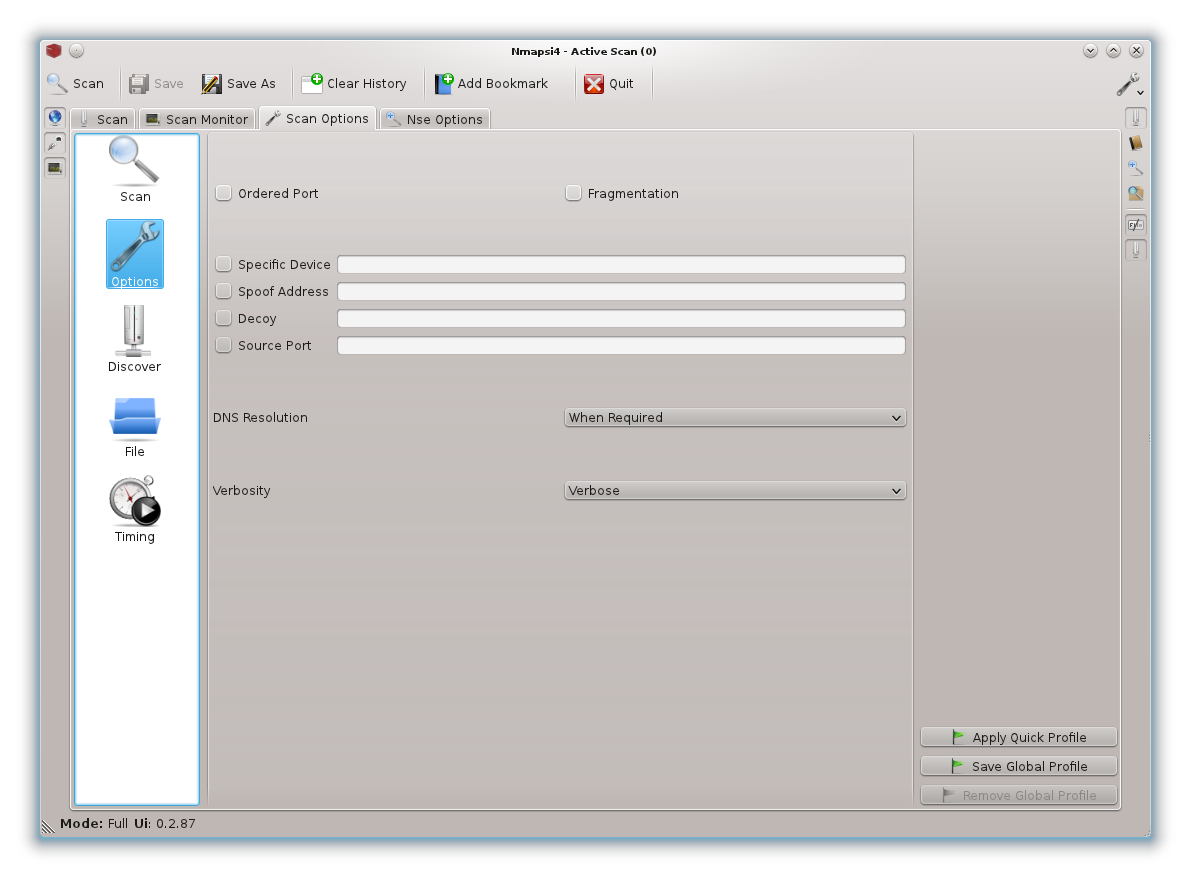
\includegraphics[width=0.7\textwidth]{22scan_options}
  \caption{Opzioni}
  \label{fig:ScanParamOptions}
\end{figure}
In questa sezione \`e possibile cambiare il livello di dettaglio, ed utilizzare 
parametri specifici come Ipv6 e frammentazione.

\subsection{Discover}
\label{sec:ScanDiscover}

\begin{figure}[h]
  \centering
  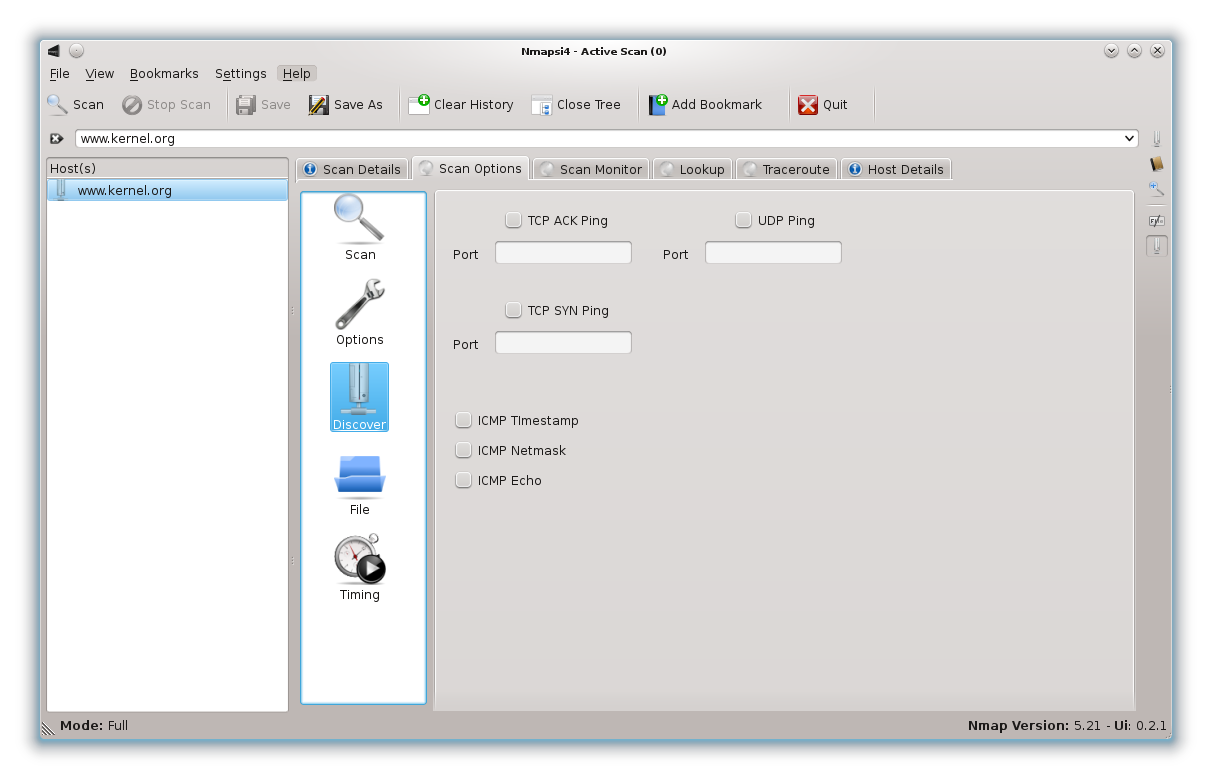
\includegraphics[width=0.7\textwidth]{23discover_scan_options}
  \caption{Discover}
  \label{fig:ScanDiscover}
\end{figure}
In questa sezione \`e possibile cambiare i parametri relativi alle tipologie di 
pacchetti da usare nella scansione.

\subsection{File}
\label{sec:ScanFile}

\begin{figure}[h]
  \centering
  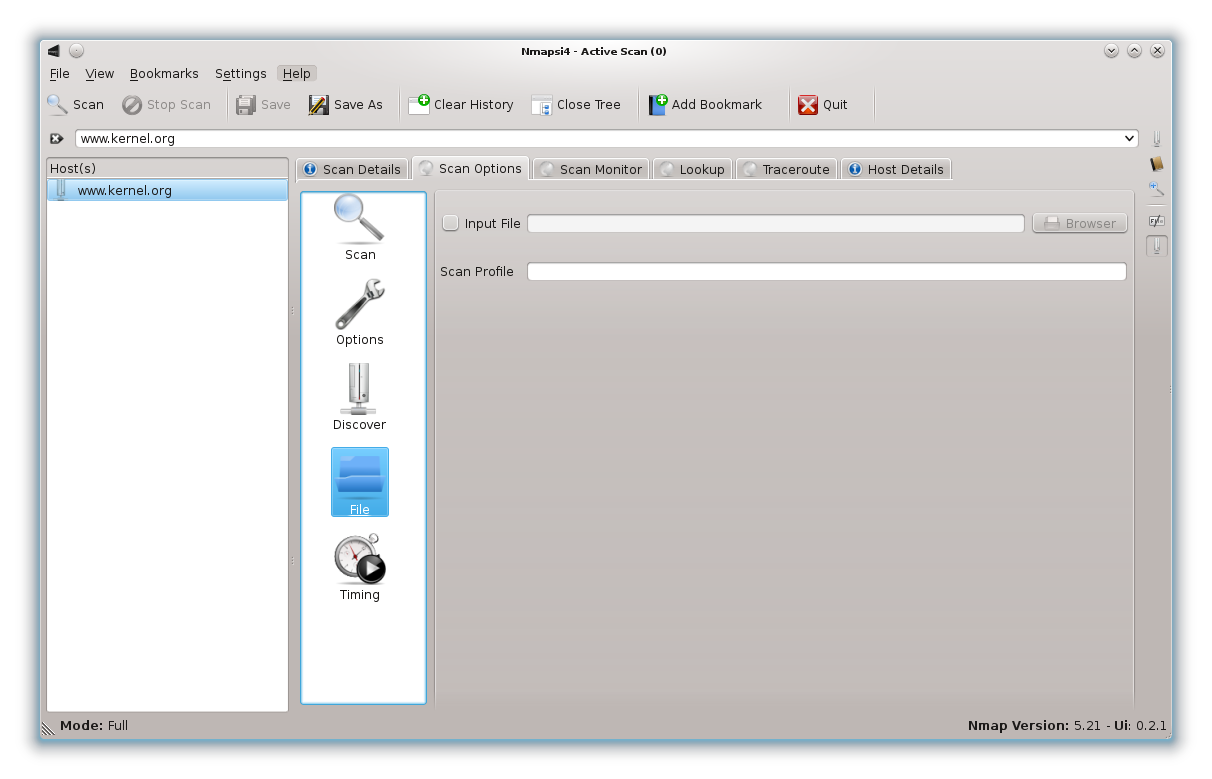
\includegraphics[width=0.7\textwidth]{24file_scan_options1}
  \caption{File}
  \label{fig:ScanFile}
\end{figure}
In questa sezione \`e possibile specificare un file di input ed un profilo 
di scansione specifico.

\subsection{Timing}
\label{sec:ScanTiming}

In questa sezione \`e possibile cambiare i parametri riguardo al tempo di 
scansione ed al TTL dei pacchetti inviati.
\begin{figure}[h]
  \centering
  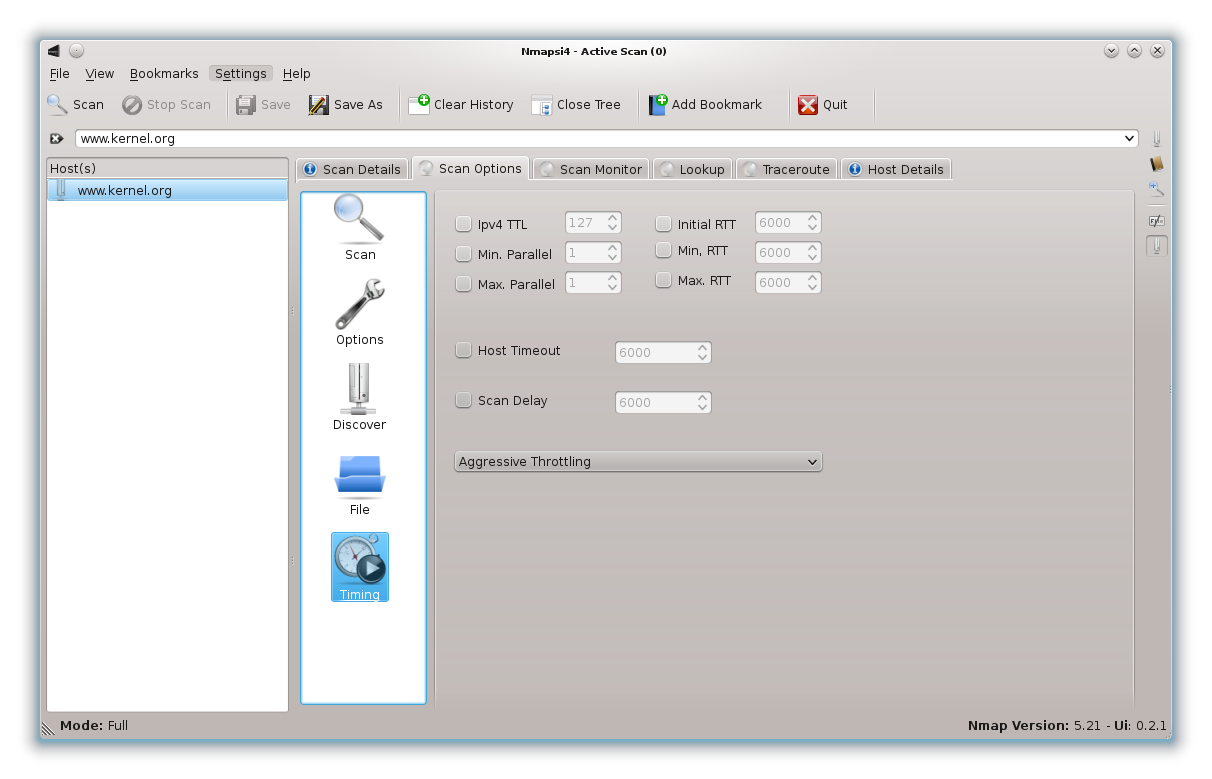
\includegraphics[width=0.7\textwidth]{25timing_scan_options2}
  \caption{Timing}
  \label{fig:ScanTiming}
\end{figure}


%%%%%%%%%%%%%%%%%%%%%%%%%%%%%%%%%%%%
\section{Monitor della Scansione}
\label{sec:ScanMonitor}
%%%%%%%%%%%%%%%%%%%%%%%%%%%%%%%%%%%%

\begin{figure}[h]
  \centering
  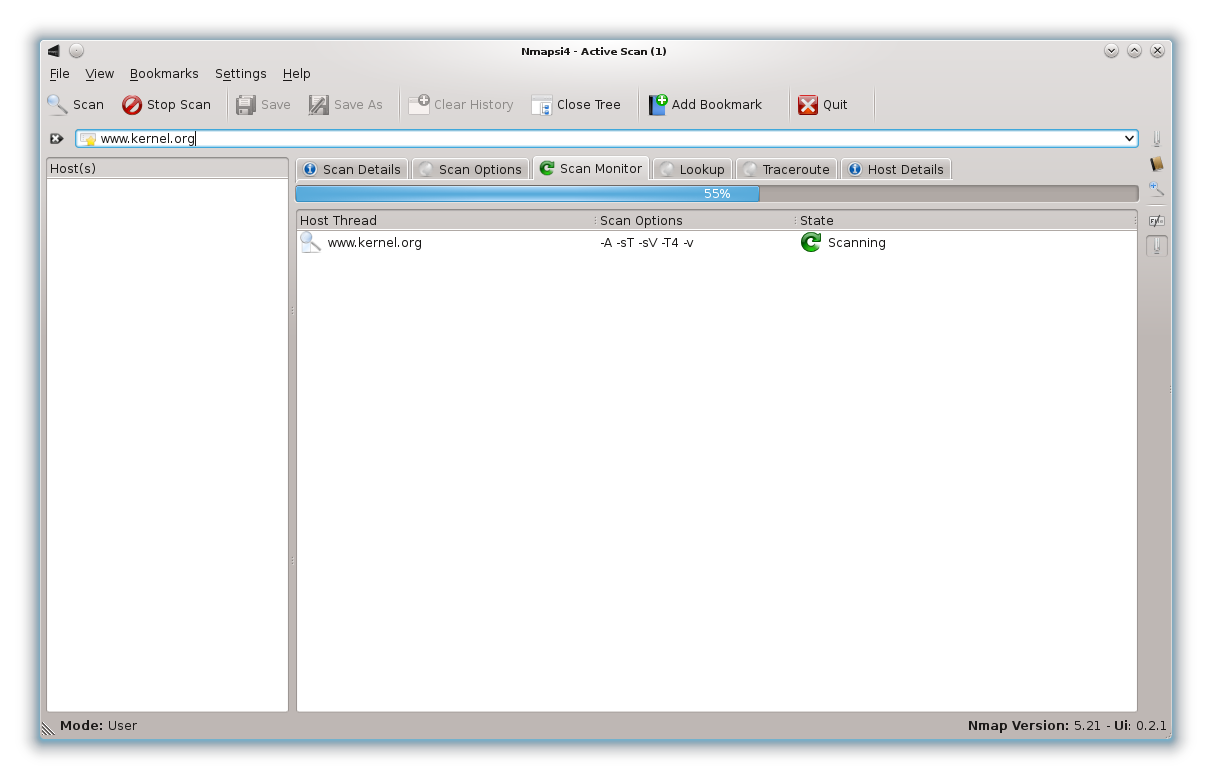
\includegraphics[width=0.7\textwidth]{scan_monitor}
  \caption{Monitor della scansione}
  \label{fig:ScanMonitor}
\end{figure}
Questa sezione elenca i vari bersagli delle scansioni attive, non ancora 
completate.

%%%%%%%%%%%%%%%%%%%%%
\section{Lookup}
\label{sec:Lookup}
%%%%%%%%%%%%%%%%%%%%%

\begin{figure}[h]
  \centering
  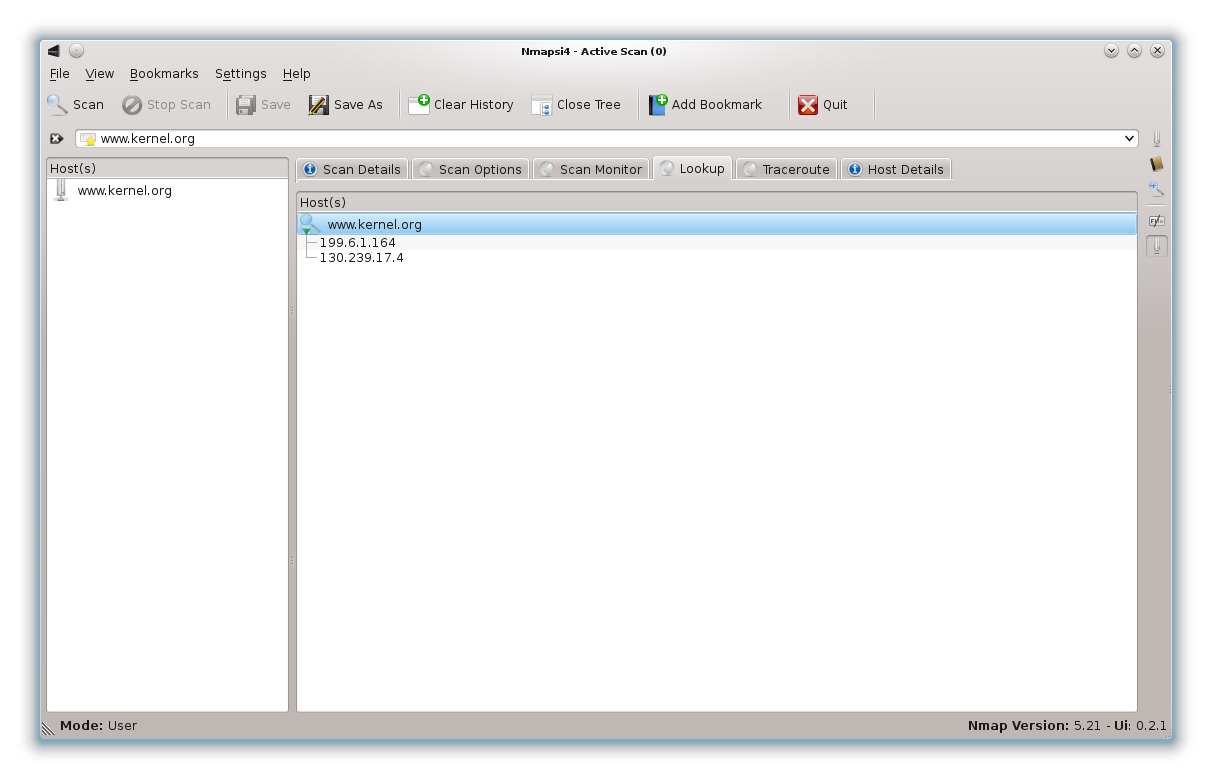
\includegraphics[width=0.7\textwidth]{4scan_lookup}
  \caption{Lookup}
  \label{fig:Lookup}
\end{figure}
Questa sezione mostra le corrispondenze tra bersagli, ip e servizi connessi.

%%%%%%%%%%%%%%%%%%%%%%%%%
\section{Traceroute}
\label{sec:Traceroute}
%%%%%%%%%%%%%%%%%%%%%%%%%

\begin{figure}[h]
  \centering
  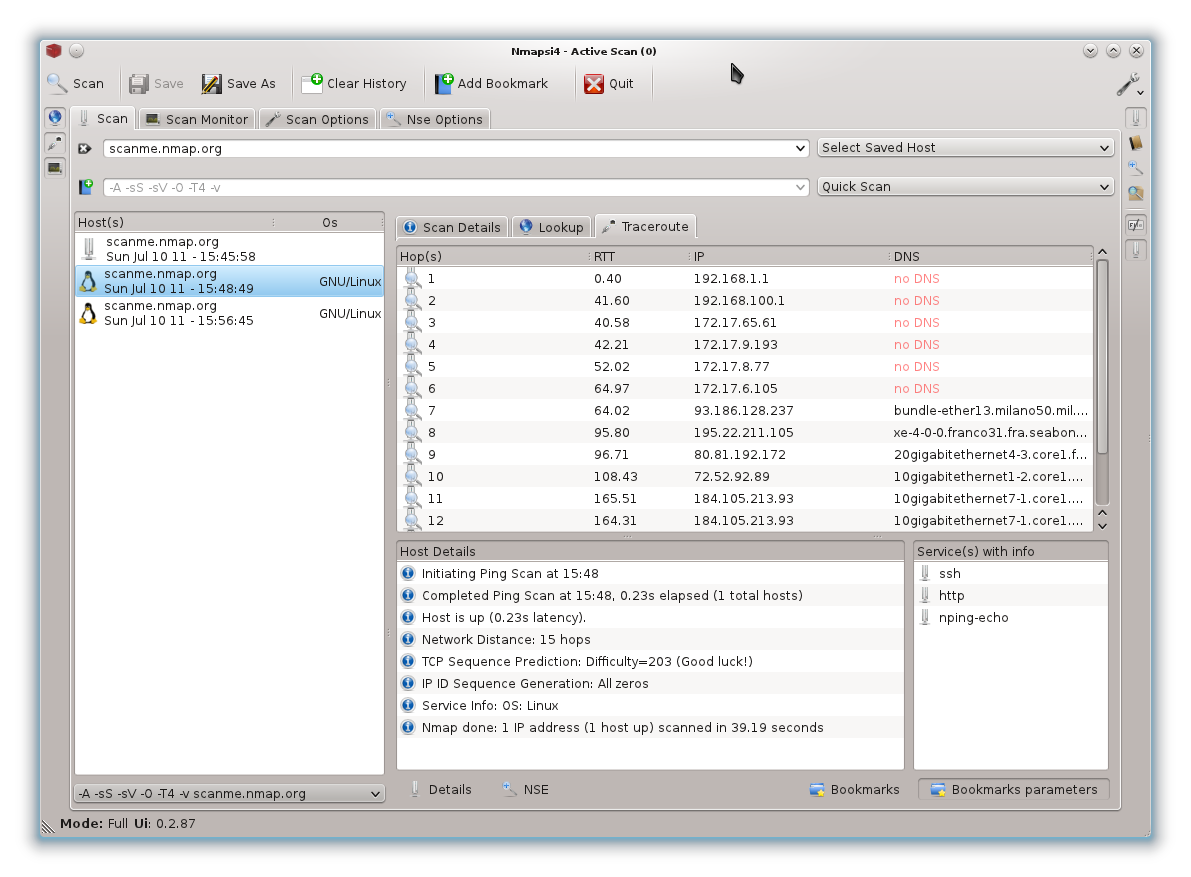
\includegraphics[width=0.7\textwidth]{5traceroute}
  \caption{Traceroute}
  \label{fig:Traceroute}
\end{figure}
Questa sezione mostra la ``strada'' percorsa dai pacchetti della scansione.

%%%%%%%%%%%%%%%%%%%%%%%%%%%
%%%%%%%%%%%%%%%%%%%%%%%%%%%
\chapter{Preferenze}
\label{ch:Preferences}
%%%%%%%%%%%%%%%%%%%%%%%%%%%
%%%%%%%%%%%%%%%%%%%%%%%%%%%

%%%%%%%%%%%%%%%%%%%%%%%%%
\section{Profili}
\label{sec:profiles}
%%%%%%%%%%%%%%%%%%%%%%%%%

\begin{figure}[h]
  \centering
  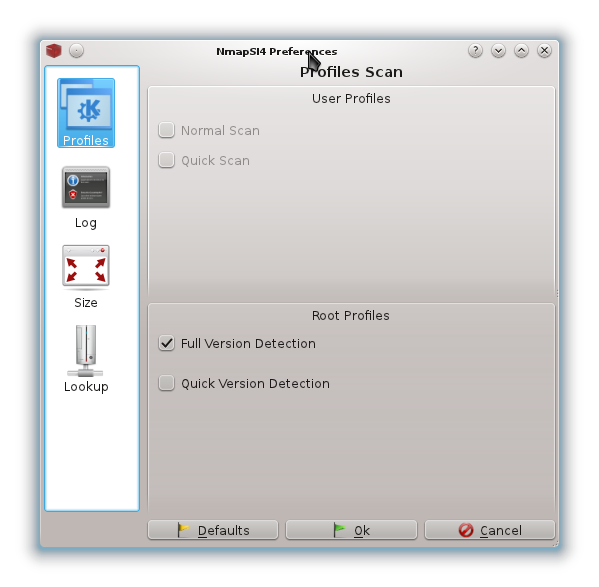
\includegraphics[width=0.6\textwidth]{1preferences_profiles}
  \caption{Profili}
  \label{fig:Profili}
\end{figure}
In questa sezione \`e possibile cambiare il profilo di scansione predefinito.

%%%%%%%%%%%%%%%%%%%
\section{Log}
\label{sec:Log}
%%%%%%%%%%%%%%%%%%%

\begin{figure}[h]
  \centering
  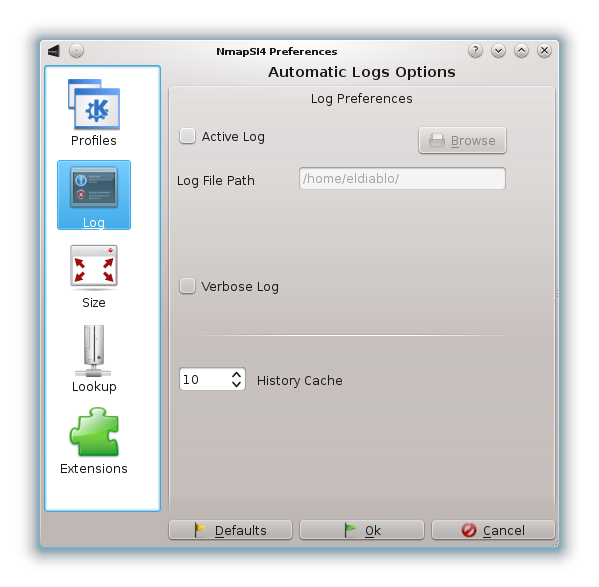
\includegraphics[width=0.6\textwidth]{2preferences_log}
  \caption{Log}
  \label{fig:Log}
\end{figure}
In questa sezione \`e possibile cambiare le impostazioni riguardanti il log 
delle scansioni.

%%%%%%%%%%%%%%%%%%%%%%%%%
\section{Dimensioni}
\label{sec:Dimensions}
%%%%%%%%%%%%%%%%%%%%%%%%%

\begin{figure}[h]
  \centering
  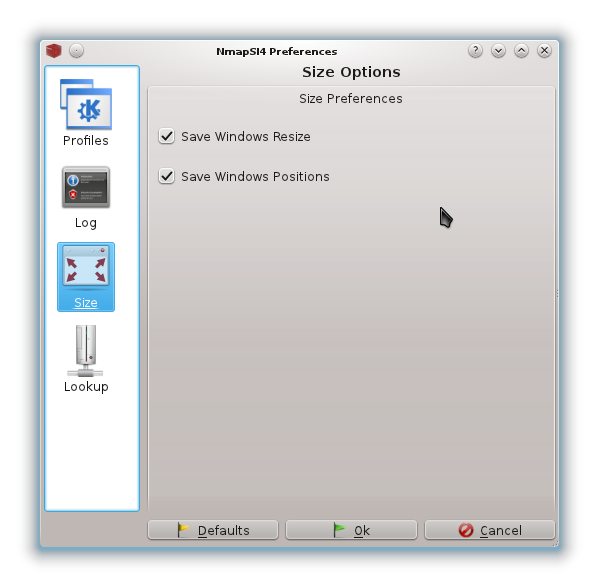
\includegraphics[width=0.6\textwidth]{3preferences_size}
  \caption{Profili}
  \label{fig:Profili}
\end{figure}
In questa sezione \`e possibile cambiare le impostazioni della finestra 
principale di NmapSI4.

%%%%%%%%%%%%%%%%%%%%%%%%%%%%%%%
\section{Lookup}
\label{sec_PreferencesLookup}
%%%%%%%%%%%%%%%%%%%%%%%%%%%%%%%

\begin{figure}[h]
  \centering
  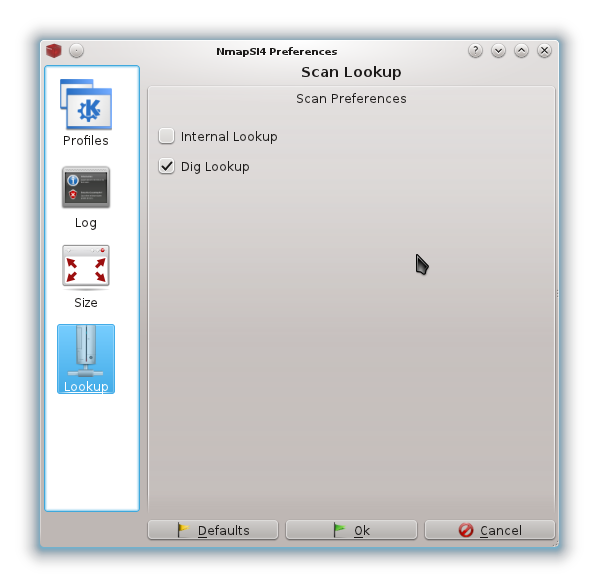
\includegraphics[width=0.6\textwidth]{4preferences_lookup}
  \caption{Lookup}
  \label{fig:PreferencesLookup}
\end{figure}
In questa sezione \`e possibile cambiare le impostazioni per il lookup.

%%%%%%%%%%%%%%%%%%%%%%%%%%%%%%%%%%
\section{Estensioni}
\label{sec:PreferencesExtensions}
%%%%%%%%%%%%%%%%%%%%%%%%%%%%%%%%%%

\begin{figure}[h]
  \centering
  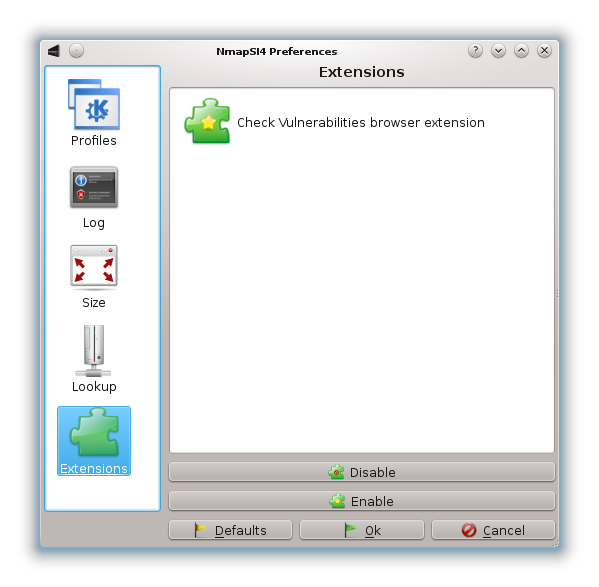
\includegraphics[width=0.6\textwidth]{5preferences_extensions}
  \caption{Estensioni}
  \label{fig:PreferencesExtensions}
\end{figure}
In questa sezione \`e possibile attivare o disattivare le estensioni di NmapSI4.

%%%%%%%%%%%%%%%%%%%%%%%%%%%%%%%%%%%%%%%%%%%%%%%%%
%%%%%%%%%%%%%%%%%%%%%%%%%%%%%%%%%%%%%%%%%%%%%%%%%
\chapter{Motore di ricerca vulnerabilit\`a}
\label{ch:Vulnerability}
%%%%%%%%%%%%%%%%%%%%%%%%%%%%%%%%%%%%%%%%%%%%%%%%%
%%%%%%%%%%%%%%%%%%%%%%%%%%%%%%%%%%%%%%%%%%%%%%%%%

%%%%%%%%%%%%%%%%%%%%%%%%%%%%%%%%%%
\section{Schermata principale}
\label{sec:VulnerabilityMain}
%%%%%%%%%%%%%%%%%%%%%%%%%%%%%%%%%%

\begin{figure}[h]
  \centering
  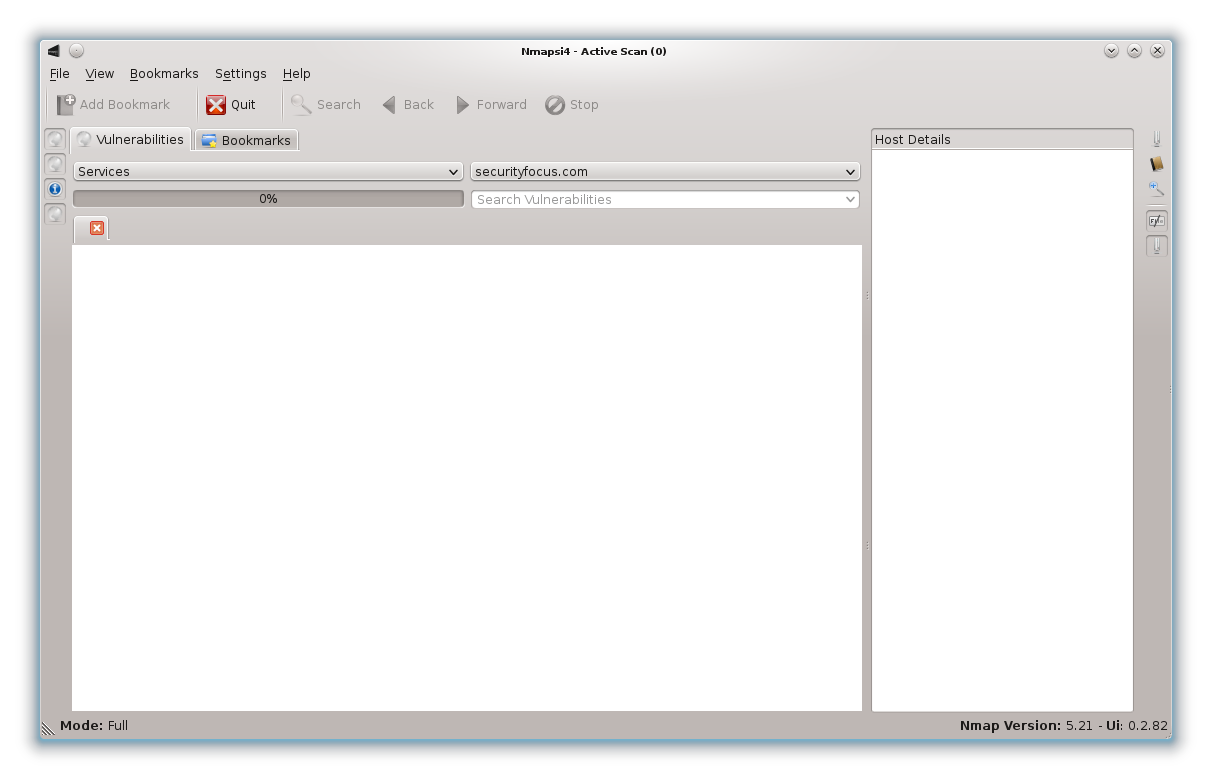
\includegraphics[width=0.7\textwidth]{vulnerabilities}
  \caption{Motore di ricerca vulnerabilit\`a}
  \label{fig:VulnerabilityMain}
\end{figure}
Questa sezione mette a disposizione un motore di ricerca per cercare eventuali 
vulnerabilit\`a dei servizi tracciati nella scansione all'interno dei maggiori 
siti di riferimento per le vulnerabilit\`a. \`E possibile cercare in base al 
servizio specifico riconosciuto tramite la scansione, oppure indicando un altro 
termine di ricerca.

%%%%%%%%%%%%%%%%%%%%%%%%%%%%%%%%%%%%%%
\section{Preferiti}
\label{sec:VulnerabilityBookmarks}
%%%%%%%%%%%%%%%%%%%%%%%%%%%%%%%%%%%%%%

\begin{figure}[h]
  \centering
  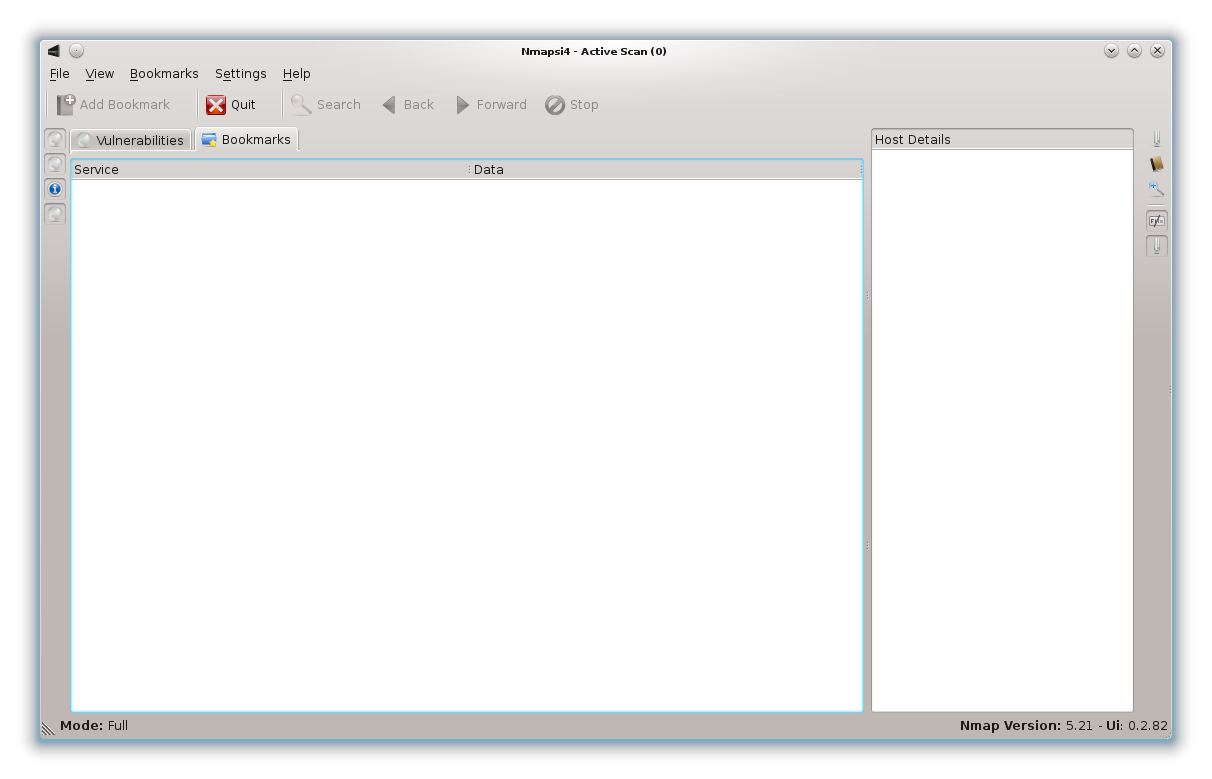
\includegraphics[width=0.7\textwidth]{vuln_bookmarks}
  \caption{Preferiti}
  \label{fig:VulnerabilityBookmarks}
\end{figure}
Qui possiamo memorizzare i nostri risultati preferiti.

%%%%%%%%%%%%%%%%%%%%%%%%%%%%%%
%%%%%%%%%%%%%%%%%%%%%%%%%%%%%%
\chapter{Log reader}
\label{ch:LogReader}
%%%%%%%%%%%%%%%%%%%%%%%%%%%%%%
%%%%%%%%%%%%%%%%%%%%%%%%%%%%%%

\begin{figure}[h]
  \centering
  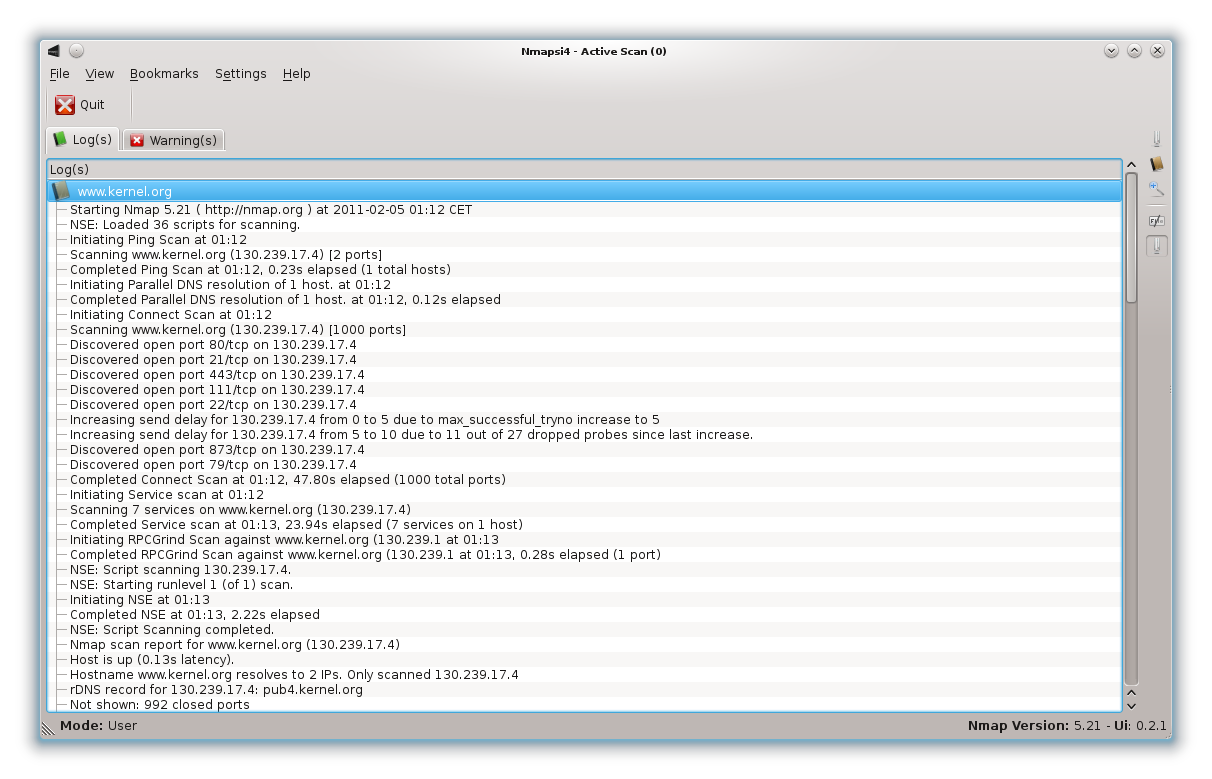
\includegraphics[width=0.7\textwidth]{log_reader}
  \caption{Log reader}
  \label{fig:LodReader}
\end{figure}
Questa sezione permette di leggere l'output completo della scansione 
effettuata da Nmap.

%%%%%%%%%%%%%%%%%%%%%%%%%%%%%%%%%%%
%%%%%%%%%%%%%%%%%%%%%%%%%%%%%%%%%%%
\chapter{Qualche esempio}
\label{ch:Examples}
%%%%%%%%%%%%%%%%%%%%%%%%%%%%%%%%%%%
%%%%%%%%%%%%%%%%%%%%%%%%%%%%%%%%%%%

%%%%%%%%%%%%%%%%%%%%%%%%%%%%%%%%%%%%%%
\section{Scansioni multiple}
\label{sec:ExamplesMultipleScan}
%%%%%%%%%%%%%%%%%%%%%%%%%%%%%%%%%%%%%%

\`E possibile usare le scansioni in diversi modi:
\begin{itemize}
\item scansione singola: \emph{ip (es. 192.168.1.1) o dns (es. www.kernel.org)}
\item scansione multipla: \emph{range di ip (es. 192.168.1.10/20) per scansionare 
  da 192.168.1.10 a 192.168.1.20}
\item scansione mista di ip e dns: \emph{es. 192.168.1.1 www.kernel.org}
\item scansione su una lista di ip o di dns: \emph{es 192.168.1.10 192.168.1.15, 
  oppure www.kernel.org www.google.com}
\end{itemize}
\textbf{\`E consigliabile non inserire un numero elevato di host da scansionare}.

%%%%%%%%%%%%%%%%%%%%%%%%%%%%%%%%%%%%%%
\section{Utilizzo dei preferiti}
\label{sec:ExamplesUseBookmarks}
%%%%%%%%%%%%%%%%%%%%%%%%%%%%%%%%%%%%%%

Per usare i preferiti basta sfruttare il pulsante in alto per aggiungerlo in lista.\\
Allo stesso modo per salvare il profilo di scansione c'\`e il pulsante posto vicino 
al form per l'inserimento dei parametri.\\
Per riusare in seguito un host o un profilo salvato, basta selezionarlo nella relativa 
schermata e selezionare ``Scansione'' per gli host o ``Usa parametri'' per i profili.\\ 
Per eliminare una voce dalla lista ripetere la procedura di riuso, scegliendo la voce di 
rimozione.
